% !TeX encoding = UTF-8
% !TeX spellcheck = es_ES
% !TeX root = ../Thermal.tex
%!TEX root=../Thermal.tex

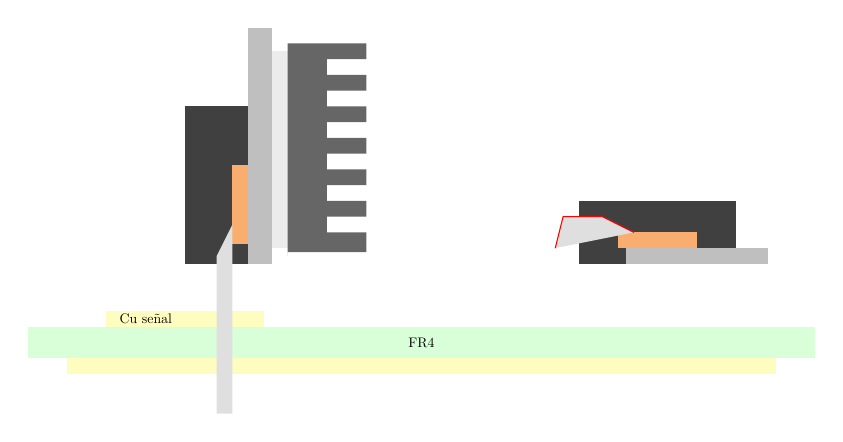
\begin{tikzpicture}[]

	\draw[draw=none,fill=green!15] (-5,-.2) rectangle +(10,.4);
	\draw[draw=none, fill=yellow!25] (-4,0.2) rectangle +(2,.2);
	\draw[draw=none, fill=yellow!25] (-4.5,-0.4) rectangle +(9,0.2);

	\node[scale=0.5] at(0,0){FR4};
	\node[scale=0.5] at (-3.5,.3){Cu señal};
\begin{scope}
	% TO-220
	\draw[draw=none,fill=black!75] (-3,1) rectangle +(.8,2);
	\draw[draw=none,fill=gray!50] (-2.2,1) rectangle + (0.3,3);
	\draw[draw=none, fill=Apricot] (-2.4,1.25) rectangle +(.2,1);
	\draw[draw=none, fill=gray!25] (-2.4,1.5) -- ++(-.2,-.4) -- ++(0,-2) -- ++(0.2,0) -- ++(0,2.4);
	\draw[draw=none,fill=gray!15] (-1.9,1.2) rectangle +(0.2,2.5);
	\draw[draw=none,fill=black!60](-1.7,1.1) -- ++(0,2.7)
	-- ++(1,0) -- ++(0,-.2) -- ++(-0.5,0) -- ++(0,-0.2)
	-- ++(0.5,0) -- ++(0,-.2) -- ++(-0.5,0) -- ++(0,-0.2)
	-- ++(0.5,0) -- ++(0,-.2) -- ++(-0.5,0) -- ++(0,-0.2)
	-- ++(0.5,0) -- ++(0,-.2) -- ++(-0.5,0) -- ++(0,-0.2)
	-- ++(0.5,0) -- ++(0,-.2) -- ++(-0.5,0) -- ++(0,-0.2)
	-- ++(0.5,0) -- ++(0,-.2) -- ++(-0.5,0) -- ++(0,-0.2)
	-- ++(0.5,0) -- ++(0,-.25) -- ++(-1,0);
\end{scope}
\begin{scope}[shift={(3,1)}]
\draw[draw=none,fill=black!75] (-1,0) rectangle +(2,.8);
\draw[draw=none,fill=gray!50] (-.4,0) rectangle +(1.8,.2);

\draw[draw=none, fill=Apricot] (-0.5,.2) rectangle +(1,.2);
\draw[red, fill=gray!25] (-0.3,.4) -- ++(-.4,0.2) 
-- ++(-.5,0) -- ++(-.1,-.4);

\end{scope}

\end{tikzpicture}